\documentclass[12pt]{article}

% Packages
\usepackage[margin=6em]{geometry} % 1 cm = 2.84528 em
\usepackage[colorlinks=true,linkcolor=red,urlcolor=blue]{hyperref}
\usepackage{algorithmicx}
\usepackage{algorithm}
\usepackage{algpseudocode}
\usepackage{stmaryrd}
\usepackage{tikz}
\usetikzlibrary{automata}
\usepackage[backend=bibtex]{biblatex}
\bibliography{sources}
\nocite{*}

\usepackage{lipsum}

% Paragraphs
\setlength{\parindent}{0em}
\setlength{\parskip}{1em}

% Includes
% Includes
\usepackage{amsfonts}
\usepackage{amsmath}
\usepackage{amssymb}
\usepackage{amsthm}
\usepackage{comment}
\usepackage[colorlinks]{hyperref}
\usepackage{letltxmacro}
\usepackage{listings}
\usepackage{stmaryrd}

% Spacing
\let\uspace\undefined
\newcommand{\uspace}{\ensuremath{\ }}

% Numbers
\let\N\undefined
\newcommand{\N}{\ensuremath{\mathbb{N}}}

\let\Z\undefined
\newcommand{\Z}{\ensuremath{\mathbb{Z}}}

\let\Zz\undefined
\newcommand{\Zz}{\ensuremath{\mathbb{Z}^{\geq 0}}}

\let\Zp\undefined
\newcommand{\Zp}{\ensuremath{\mathbb{Z}^{+}}}

\let\Q\undefined
\newcommand{\Q}{\ensuremath{\mathbb{Q}}}

\let\R\undefined
\newcommand{\R}{\ensuremath{\mathbb{R}}}

\let\Rz\undefined
\newcommand{\Rz}{\ensuremath{\mathbb{R}^{\geq 0}}}

\let\Rp\undefined
\newcommand{\Rp}{\ensuremath{\mathbb{R}^{+}}}

\let\C\undefined
\newcommand{\C}{\ensuremath{\mathbb{C}}}

\let\mcal\undefined
\newcommand{\mcal}[1]{\ensuremath{\mathcal{#1}}}

\let\mbb\undefined
\newcommand{\mbb}[1]{\ensuremath{\mathbb{#1}}}

% Grouping
\let\parens\undefined
\newcommand{\parens}[1]{\ensuremath{\left(#1\right)}}

\let\brackets\undefined
\newcommand{\brackets}[1]{\ensuremath{\left[#1\right]}}

\let\braces\undefined
\newcommand{\braces}[1]{\ensuremath{\left\{#1\right\}}}

\let\angles\undefined
\newcommand{\angles}[1]{\ensuremath{\left\langle#1\right\rangle}}

\let\ceil\undefined
\newcommand{\ceil}[1]{\ensuremath{\left\lceil#1\right\rceil}}

\let\floor\undefined
\newcommand{\floor}[1]{\ensuremath{\left\lfloor#1\right\rfloor}}

% Sets and Function Spaces
\let\type\undefined
\newcommand{\type}[3]{\ensuremath{#1 \colon #2 \to #3}}

\let\powset\undefined
\newcommand{\powset}[1]{\ensuremath{2^{#1}}}

\let\mod\undefined
\newcommand{\mod}{\ensuremath{\uspace\mathrm{mod}\uspace}}

\let\ker\undefined
\newcommand{\ker}{\ensuremath{\mathrm{ker}}}

\let\dom\undefined
\newcommand{\dom}{\ensuremath{\mathrm{dom}}}

\let\ran\undefined
\newcommand{\ran}{\ensuremath{\mathrm{ran}}}

\let\im\undefined
\newcommand{\im}{\ensuremath{\mathrm{im}}}

\let\coker\undefined
\newcommand{\coker}{\ensuremath{\mathrm{coker}}}

\let\codim\undefined
\newcommand{\codim}{\ensuremath{\mathrm{codim}}}

% Complex Numbers
\let\Re\undefined
\newcommand{\Re}{\ensuremath{\mathrm{Re}}}

\let\Im\undefined
\newcommand{\Im}{\ensuremath{\mathrm{Im}}}

% Probability
\let\Pr\undefined
\newcommand{\Pr}{\ensuremath{\mathrm{Pr}}}

\let\E\undefined
\newcommand{\E}{\ensuremath{\mathrm{E}}}

\let\Var\undefined
\newcommand{\Var}{\ensuremath{\mathrm{Var}}}

\let\Cov\undefined
\newcommand{\Cov}{\ensuremath{\mathrm{Cov}}}

% Integrals
\let\dee\undefined
\newcommand{\dee}[1]{\ensuremath{\uspace d #1}}

% Linear Algebra
\let\abs\undefined
\newcommand{\abs}[1]{\ensuremath{\left\lvert#1\right\rvert}}

\let\norm\undefined
\newcommand{\norm}[1]{\ensuremath{\left\lVert#1\right\rVert}}


% Computational Complexity
\let\class\undefined % Complexity class
\newcommand{\class}[1]{\ensuremath{\mathbf{#1}}}

\let\prob\undefined % Complexity problem
\newcommand{\prob}[1]{\ensuremath{\text{#1}}}

% Theorem environment
\theoremstyle{plain}
\newtheorem{theorem}{Theorem}

\theoremstyle{plain}
\newtheorem{lemma}{Lemma}

\theoremstyle{plain}
\newtheorem{claim}{Claim}

\theoremstyle{plain}
\newtheorem{fact}{Fact}

\theoremstyle{plain}
\newtheorem{remark}{Remark}

\theoremstyle{plain}
\newtheorem{definition}{Definition}

\theoremstyle{plain}
\newtheorem{example}{Example}

\theoremstyle{plain}
\newtheorem{question}{Question}

% Code environment
\lstdefinestyle{plainsty}{
  basicstyle=\small\ttfamily,
  language=C,
  xleftmargin=\parindent,
  aboveskip=1em,
  belowskip=1em,
  showspaces=false,
  showstringspaces=false,
  keywordstyle = {},
}

\lstnewenvironment{pcode}{\lstset{style=plainsty}}{}

\let\pinl\undefined
\newcommand{\pinl}{\lstinline[style=plainsty]}

\newcommand*{\SavedLstInline}{} % Allows plain code usage in math mode.
\LetLtxMacro\SavedLstInline\pinl
\DeclareRobustCommand*{\pinl}{%
  \ifmmode
    \let\SavedBGroup\bgroup
    \def\bgroup{%
      \let\bgroup\SavedBGroup
      \hbox\bgroup
    }%
  \fi
\SavedLstInline}

\let\ttcode\undefined
\newcommand{\ttcode}[1]{\small{\texttt{#1}}}


% Text markings

\let\tturl\undefined
\newcommand{\tturl}[1]{\href{#1}{\texttt{#1}}}

\let\red\undefined
\newcommand{\red}[1]{\textbf{\color{red}#1}}


% Abbreviations
\let\st\undefined
\newcommand{\st}{\ensuremath{\uspace\colon\uspace}}

\let\ow\undefined
\newcommand{\ow}{\ensuremath{\text{otherwise}}}




\let\company\undefined
\newcommand{\company}{\textbf{Big Tech Company}}

\let\Android\undefined
\newcommand{\android}{Android}

\let\state\undefined
\newcommand{\state}{\ensuremath{\sigma}}

\let\var\undefined
\newcommand{\var}{\ensuremath{x}}

\let\domval\undefined
\newcommand{\domval}{\ensuremath{\mathcal{A}}}

\let\formula\undefined
\newcommand{\form}{\ensuremath{\varphi}}

\let\domform\undefined
\newcommand{\domform}{\ensuremath{\mathcal{F}}}

% Author
\title{The Dangerous Graph}
\author{Anton Xue}
% \date{\today}
\date{}

% Document
\begin{document}
\maketitle

\subsection{Real-World Applications?}

A friend working at \company{} told to me about a problem
they were working on:
how can we have automated detection of crashing
errors in \android{} applications?

Users interacts with \android{} applications by touching
the phone's user interface (UI).
Touching the UI in specific ways alters the internal state of the application.
The UI is specified by XML files that (each?) represent a
different display layout.
When specific touches are performed, different displays may be shown.
These display transitions are conditional on the internal state of the
application and the current active display.

We then ask:
\textbf{what sequence of actions will cause the application to crash?}


\subsection{Defining the Problem}
From a high-level perspective, the problem is not well-defined in part
because we have not discussed the level of access we have to the
application under testing.
Are we given the source code?
Can we monitor internal application state and variables during execution?
Or are we given just the phone and told to play with it?

If we have access to the source code, we may apply techniques such as
backwards symbolic execution~\cite{baldoni-backwards} or
slicing~\cite{weiser-slicing}.

If we may monitor application state during execution through some debugger
or trace dumper, then short of decompilation, we may try techniques such
as randomized testing or somehow approximating behavior.

If we are given just a phone, then we throw it against a wall.

The first condition presented, with complete source code access, is of
course, the most favorable.
It is also the biggest headache because all the techniques listed are
a pain to implement.

We opt for the second.

\subsection{Modeling the Problem}
\begin{definition}[Tail and Head Set]
For a directed multigraph $G = \parens{V, E}$,
where each edge has form $e = \parens{u, v} \in E$ with tail $u$ and head $v$,
we define the \textit{tail set} $T_u$ and \textit{head set} $H_v$:
\begin{align*}
  T_u &= \setcomp{\parens{u, v}}{\exists v \st \parens{u, v} \in E} \\
  H_v &= \setcomp{\parens{u, v}}{\exists u \st \parens{u, v} \in E}
\end{align*}
$\square$
\end{definition}

This allows us to abbreviate some notation when reasoning about multigraphs.

\begin{definition}[Application Graph]
An \textit{application graph} is a directed multigraph $G = \parens{V, E}$,
where each edge is labeled with a formula $e_{\form}$ in some logical
theory $\domform$ such that:
\begin{enumerate}
  \item[(1)]
    The formula associated with each edge in a tail set is disjoint:
    \begin{align*}
      \forall u \in V,
      \forall e_i, e_j \in E_u
      \colon
      e_{i, \form} \land e_{j, \form} \implies \bot
    \end{align*}

  \item[(2)]
    The disjunction of each edge in a tail set is a tautology:
    \begin{align*}
      \forall u \in V
      \colon
      \parens{\bigvee_{e \in E_u} e_{\form}} \implies \top
    \end{align*}
\end{enumerate}
$\square$
\end{definition}

Here, every vertex corresponds to some display.
Every edge $e$ is intended to represent an action, and the associated
formula $e_{\form}$ attached to each edge is intended ot capture the
logical conditions that must be satisfied when the action is performed
so that the transition may take place.
We require that the formula associated for each action be disjoint logical
formulae, meaning that their conjunction is not satisfiable.
This ensures uniqueness of action.


\begin{example}[Simple UI]
Testing the limits of our \LaTeX{} powers, we bring you this example.
Here, the application consists of three displays, each with tree elements:

\begin{itemize}
  \item
    A {\color{blue} blue $n$-value label} that shows the global value of $n$.

  \item
    A {\color{green} green action buton} that modifies $n$ according
    to its description.

  \item
    A {\color{red} red warp button} that moves between displays.
    Sometimes crashes.
\end{itemize}

I think the {\color{green} green color} hurts my eyes to read.
{\color{red} Oof owie ouch!}

\begin{minipage}{0.45\textwidth}
  \begin{center}
  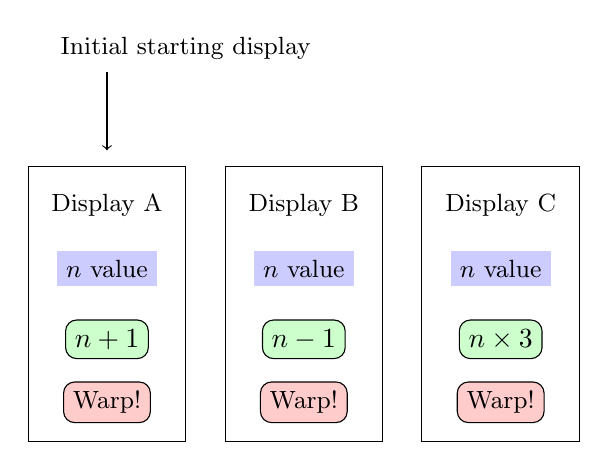
\begin{tikzpicture}
    \draw (0.0, 0.0) -- (2.0, 0.0) -- (2.0, 3.5) -- (0.0, 3.5) -- (0.0, 0.0);
    \draw (2.5, 0.0) -- (4.5, 0.0) -- (4.5, 3.5) -- (2.5, 3.5) -- (2.5, 0.0);
    \draw (5.0, 0.0) -- (7.0, 0.0) -- (7.0, 3.5) -- (5.0, 3.5) -- (5.0, 0.0);

    \node[] at (1.0, 3.0) {{\small Display A}};
    \node[] at (3.5, 3.0) {{\small Display B}};
    \node[] at (6.0, 3.0) {{\small Display C}};

    \node[fill=blue!20] at (1.0, 2.2) {{\small $n$ value}};
    \node[fill=blue!20] at (3.5, 2.2) {{\small $n$ value}};
    \node[fill=blue!20] at (6.0, 2.2) {{\small $n$ value}};

    \node[fill=green!20,draw,rounded corners] at (1.0, 1.3) {$n + 1$};
    \node[fill=green!20,draw,rounded corners] at (3.5, 1.3) {$n - 1$};
    \node[fill=green!20,draw,rounded corners] at (6.0, 1.3) {$n \times 3$};

    \node[fill=red!20,draw,rounded corners] at (1.0, 0.5) {{\small Warp!}};
    \node[fill=red!20,draw,rounded corners] at (3.5, 0.5) {{\small Warp!}};
    \node[fill=red!20,draw,rounded corners] at (6.0, 0.5) {{\small Warp!}};

    \node[] at (2.0, 5.0) {{\small Initial starting display}};

    \draw[->] (1.0, 4.7) -- (1.0, 3.7);

  \end{tikzpicture}
  \end{center}
\end{minipage}
\hfill
\begin{minipage}{0.5\textwidth}
\begin{pcode}
// Display A:
green: set n = n + 1
red:   if n mod 5 == 1 then go to B
       if n mod 5 == 2 then go to C
       otherwise do nothing
// Display B:
green: set n = n - 1
red:   if n mod 5 == 0 then go to A
       if n mod 5 == 2 then go to C
       otherwise do nothing
// Display C:
green: set n = n * 3
red:   if n mod 5 == 0 then go to A
       if n mod 5 == 1 then go to B
       otherwise CRASH
\end{pcode}
\end{minipage}

The application graph should then look something like:

\let\redP\undefined
\newcommand{\redP}{\ensuremath{{\color{red} \textit{red}}}}

\let\greenP\undefined
\newcommand{\greenP}{\ensuremath{{\color{green} \textit{green}}}}

\begin{center}
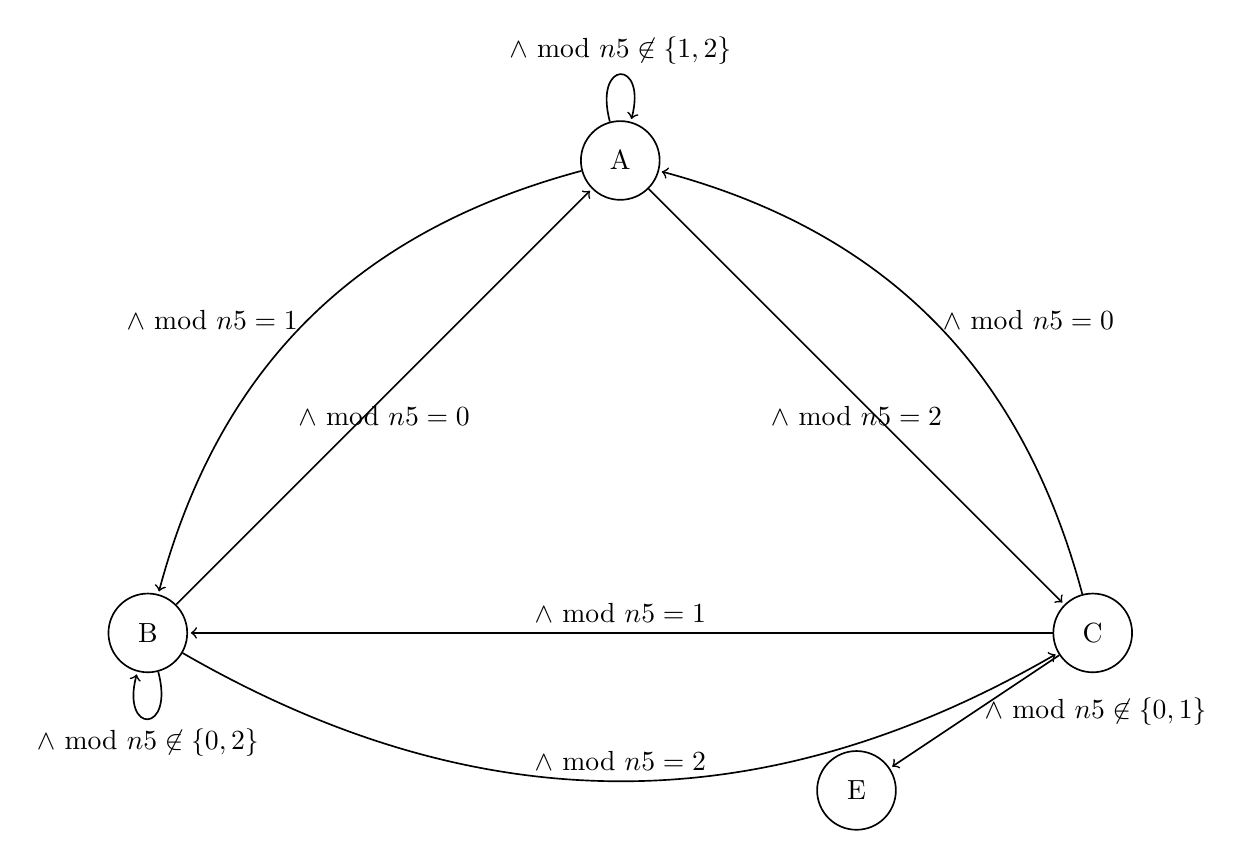
\begin{tikzpicture}
  [->,
   % >=stealth',
   shorten >=1pt,
   auto,
   node distance=3cm,
   semithick,
   state/.style={circle, draw, minimum size=1cm} 
  ]
  \node[state] (B) at (0, 1)  {B};
  \node[state] (C) at (12, 1) {C};
  \node[state] (A) at (6, 7)  {A};
  \node[state] (E) at (9, -1) {E};

  \path (A) edge [loop above] node
      {$\redP \land \mod{n}{5} \not\in \braces{1, 2}$} (A);
  
  \path (A) edge [bend right, left] node
      {$\redP \land \mod{n}{5} = 1$} (B);

  \path (A) edge [below] node
      {$\redP \land \mod{n}{5} = 2$} (C);

  \path (B) edge [loop below] node
      {$\redP \land \mod{n}{5} \not\in \braces{0, 2}$} (B);

  \path (B) edge [below] node
      {$\redP \land \mod{n}{5} = 0$} (A);

  \path (B) edge [bend right] node
      {$\redP \land \mod{n}{5} = 2$} (C);

  \path (C) edge [bend right, right] node
      {$\redP \land \mod{n}{5} = 0$} (A);

  \path (C) edge [above] node
      {$\redP \land \mod{n}{5} = 1$} (B);

  \path (C) edge [right] node
      {$\redP \land \mod{n}{5} \not\in \braces{0, 1}$} (E);
\end{tikzpicture}
\end{center}

Here $\redP$ denotes the action of the red button getting pressed.
This is a mess, but I hope the idea is clear: the objective of the application
grpah is to captur ethe notion of the conditions on which transitions are
made when actions are performed.
All actions as button presses, for the sake of simplicity.
We treat the error crashing as a separate display.

We chose not to draw the green button presses $\greenP$ because otherwise
the graph would be super cluttered.
Actions that do not bring you to a new display are treated as self-loops.
Hence, all $\greenP$ would just be self-loops.
$\square$
\end{example}

\subsection{The Dangerous Game}

Here is how we play The Dangerous Game:
\textbf{starting from an empty graph of just vertices,
how can we construct all the edges with the correct formula
attached to each edge?}

To play the dangerous game to begin with, we have to keep
track of some notion of current state of variable values:
\begin{definition}[Exploration State]
An exploration state is a pairing $\parens{G, \state}$,
where $G$ is an application graph, and $\state$ is a mapping of all relevant
program variables that appear in the graph to values in some
domain $\domval$.
\end{definition}

What are the values in $\domval$?
For now, we imagine them as logical formulae over the range of values that
each variable may have with respect to their typings.
Another reason for strong, static typing, yah?

There are some difficulties:
it may be impossible to, without knowing
the source code, to guess all the conditions that the programmer decided
to encode for making the buttons transition.
Nevertheless, we can try some basic, basic exploration techniques.


\begin{algorithm}[H]
\caption{Naive exploration algorithm}
\begin{algorithmic}[1]
\Procedure{Naive Exploration}{$G = \parens{V, E}$}
  \State Let $v_0$ be the starting vertex in $G$
  \State $v \mapsfrom v_0$
  \While{timer or ticker of some sort has not run out}
    \State Click the next button in display $v$ according to some
           deterministic selection.
    \If{this transitions us to a new display $v^\prime$}
      \State 
      \State $v \mapsfrom v^\prime$
    \EndIf
  \EndWhile
\EndProcedure
\end{algorithmic}
\end{algorithm}



\subsection{Conclusion}


\printbibliography


\end{document}
